\documentclass[10pt]{beamer}

%STANDARD PREAMBLE
%https://tex.stackexchange.com/questions/68821/is-it-possible-to-create-a-latex-preamble-header
\usepackage{/Users/mwojno01/Repos/latex_preamble/beamer_preamble}

% DOCUMENT SPECIFIC STUFF
% using default arg uments; see https://stackoverflow.com/questions/1812214/latex-optional-arguments




%%%% Citations should be rendered differently in beamer -- ADD TO BEAMER

\title{Integrating survival functions}

\begin{document}

\maketitle

\begin{frame}{Survival functions}
\begin{center}
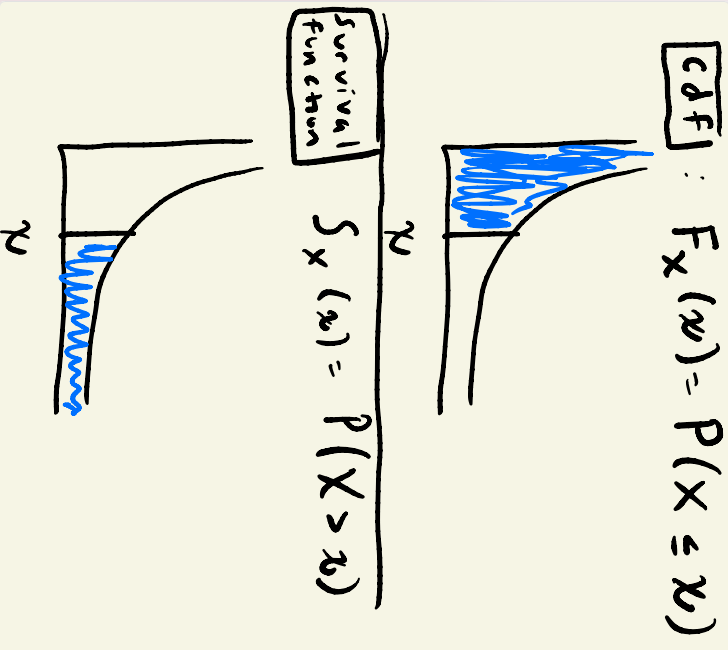
\includegraphics[width=.5\textwidth, angle=90]{images/cdf_and_survival_function}
\end{center}
\pause 
\vfill 
\textbf{Question}: What is the meaning of
\[ \int_0^\infty S_X(x) \, dx = \int_{0}^\infty P(X >x) \, dx\]  
\end{frame}


\begin{frame}{Survival functions}
\begin{center}
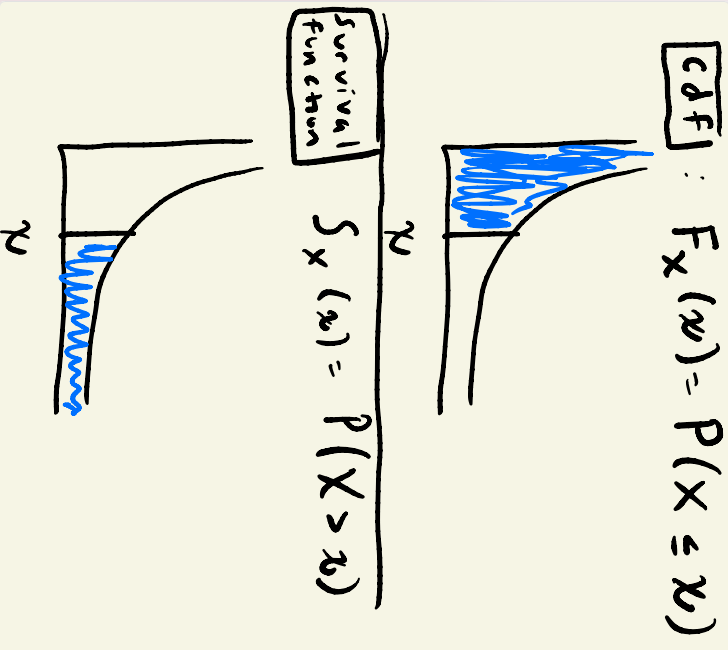
\includegraphics[width=.5\textwidth, angle=90]{images/cdf_and_survival_function}
\end{center}
\vfill 
\textbf{Answer}: If $X$ is non-negative,
\[ \int_{0}^\infty P(X >x) \, dx = \E[X] \quad !!! \] 
\[ \text{\alert{Why?}} \]
\end{frame}

\begin{frame}[standout]
We will use measure theory to make the relationship intuitive.
\end{frame}


\section{Review: General integration}
\begin{frame}{Integrals of simple functions}

\begin{definition}
Let $h$ be simple, say $h = \sum_{i=1}^r y_i I_{A_i}$ where the $A_i$ are disjoint sets in $\F$.  Then
\begin{align*}
\ds\int_{\Omega} h \wrt{\mu} := \ds\sum_{i=1}^r y_i \; \mu(A_i).
\labelit \label{eqn:integral_of_simple_function}	
\end{align*}
 \label{def:integral_of_simple_function}
\end{definition}

\begin{figure}[H]
\centering 
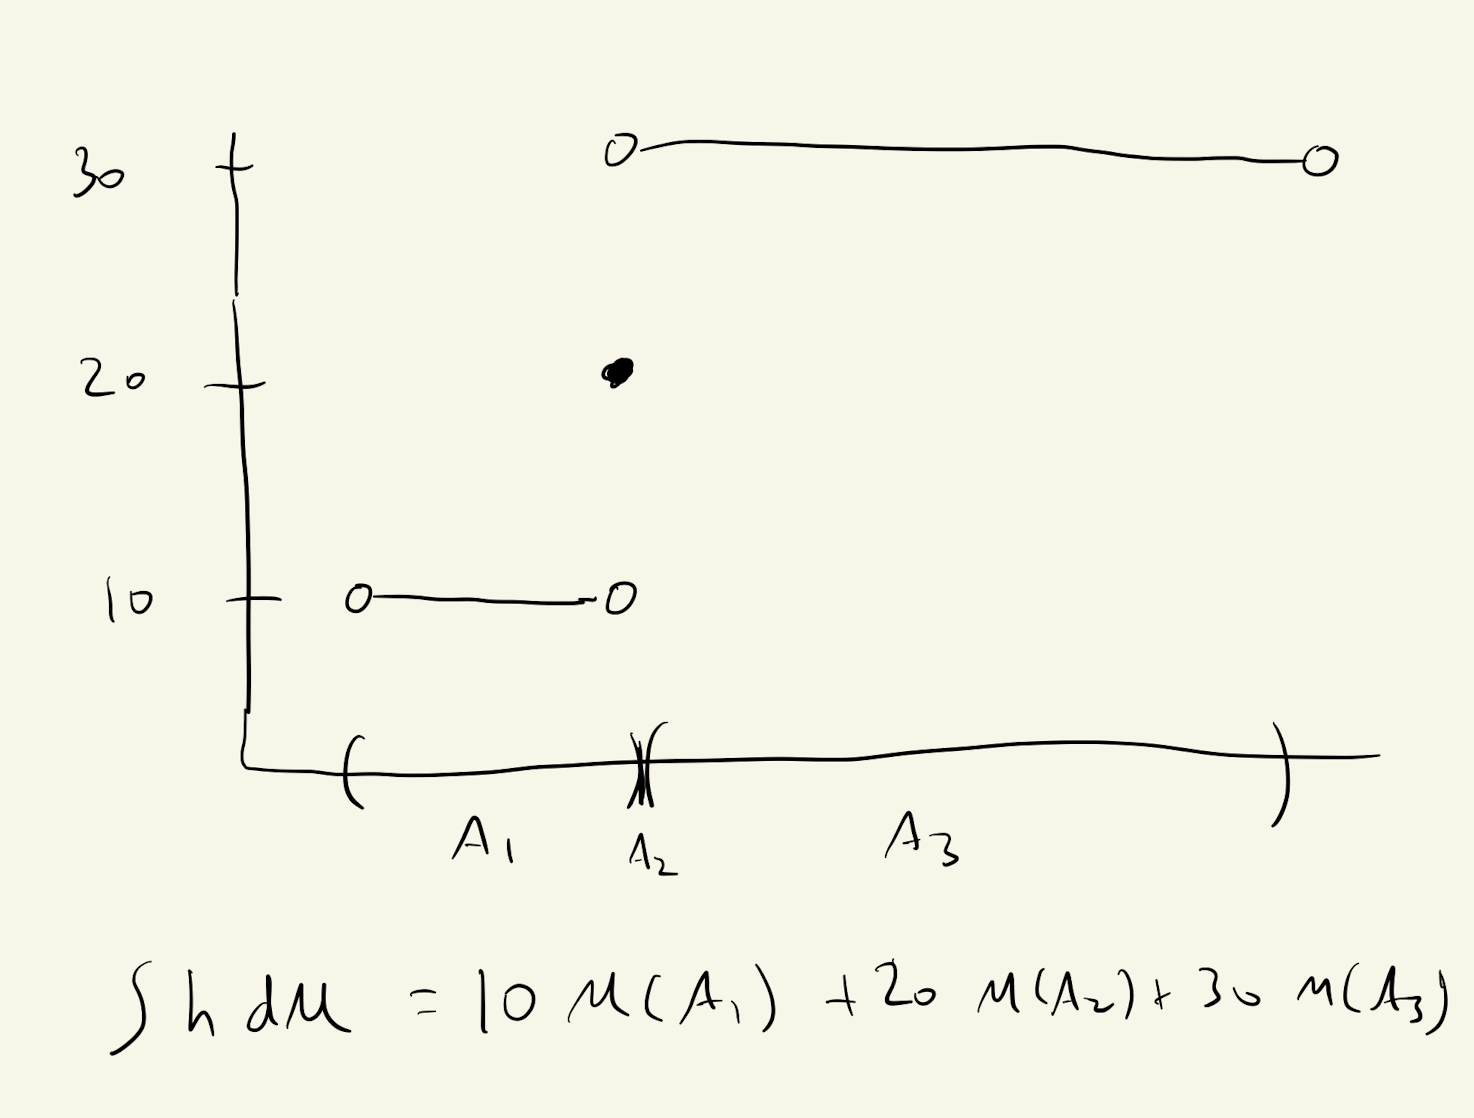
\includegraphics[width=.4\textwidth]{images/integral_of_simple_function}	
%\caption{The Lesbesgue integral of a simple function. {\scriptsize (In this case, the simple function is also a step function.)}}
\end{figure}	

{\tiny Note: The integral of a simple function exists whenever $\infty$ and  $-\infty$ do not both appear in the sum. } \\
\pause 
{\tiny Note: An example of when we'd want to use some $\mu$ other than Lebesgue measure will come up shortly!} 
\end{frame}

\begin{frame}{Integrals of non-negative Borel measurable functions}
\begin{definition}

If $h$ is non-negative Borel measurable, we define 

\[  \ds\int_{\Omega} h \wrt{\mu} = \sup \bigg\{ \ds\int_{\Omega} s \wrt{\mu} : s \quad \text{simple,} \quad 0 \leq s \leq h  \bigg\} \]
\label{def:integral_of_non_negative_Borel_measurable_function}
\end{definition}


\begin{figure}[H]
\centering
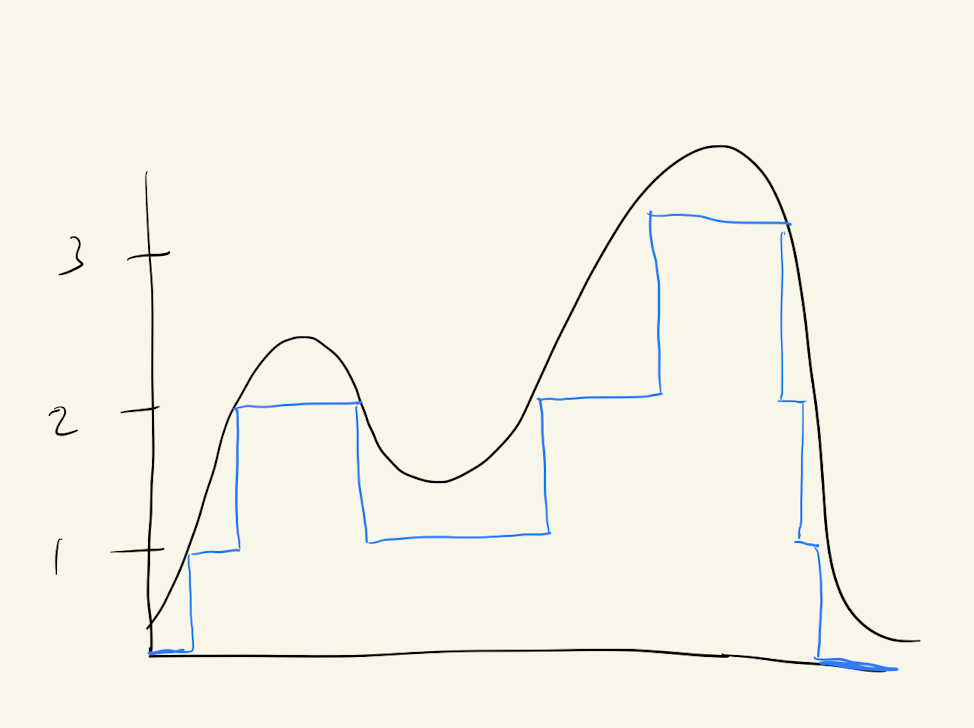
\includegraphics[width=.4\textwidth]{images/simple_function_approximating_non_negative_function}	
%\caption{A simple function approximating a non-negative function in terms of its integral}
\end{figure}

\bottomtext{The integral of a non-negative Borel measurable function \textit{always} exists (although it may take on the value $+\infty$).}
\end{frame}

%\begin{frame}{Integrals of arbitrary Borel measurable functions}
%
%Let $h$ be an arbitrary Borel measurable function.   We will express an arbitrary Borel measurable function as as the difference of two non-negative Borel measurable functions.
%
%
%\begin{figure}[H]
%\centering
%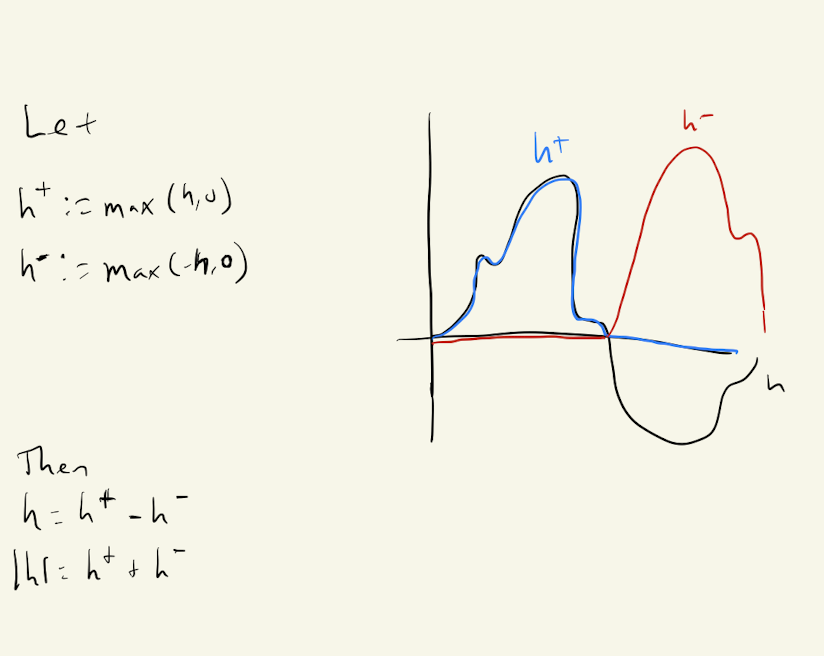
\includegraphics[width=.4\textwidth]{images/arbitrary_borel_measurable_functions_in_terms_of_nonnegative_borel_measurable_functions}
%\end{figure}
%
%We can define the integral of $h$ by 
%
%\[ \ds\int_\Omega h \wrt{\mu} = \ds\int_\Omega h^+ \wrt{\mu} - \ds\int_\Omega h^- \wrt{\mu} \]
%
%\vfill
%
%\bottomtext{The integral of an arbitrary non-negative Borel function exists so long as it does not take the form $+\infty - \infty$.} 
%
%\end{frame}


\section{Resolution}

\begin{frame}{Different ways to measure ``area under the curve"}
\begin{center}
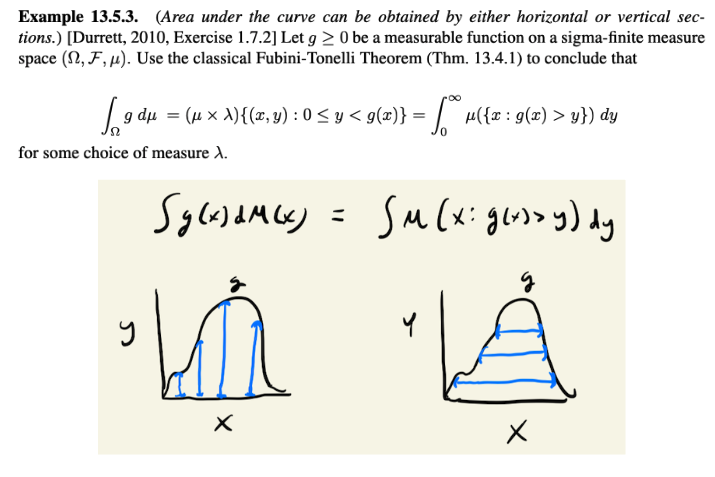
\includegraphics[width=1.0\textwidth]{images/auc_via_either_horizontal_or_vertical_sections}
\end{center}
\end{frame}

%\begin{frame}{Resolution}
%From the last slide, it is intuitive that
%\[  \int_\Omega g \wrt{\mu} = \int_0^\infty \mu(\set{x : g(x) > y}) \wrt{y} \]
%\vfill 
%Through a simple renotation
%\begin{align*}
%\mu \rightarrow P \; \text{(measure)}& \quad\quad x \rightarrow \omega \; \text{(horizontal axis label)} \\
%g \rightarrow X \; \text{(function)} & \quad\quad y \rightarrow x 	 \; \text{(vertical axis label)}
%\end{align*}
%\vfill 
%we obtain
%\begin{align*}
% \vertequalto{\int_\Omega X \wrt{P}}{\E[X]} =  \vertequalto{\int_0^\infty P(\set{\omega : X(\omega) > x}) \wrt{x}}{\int_0^\infty P(X > x) \wrt{x}}
%\end{align*}
%\end{frame}

\begin{frame}{Resolution}
Taking $g(x)=x$ and $\mu = P_X$ to be a probability measure on $(\R,\B(\R))$, we obtain 

\begin{figure}
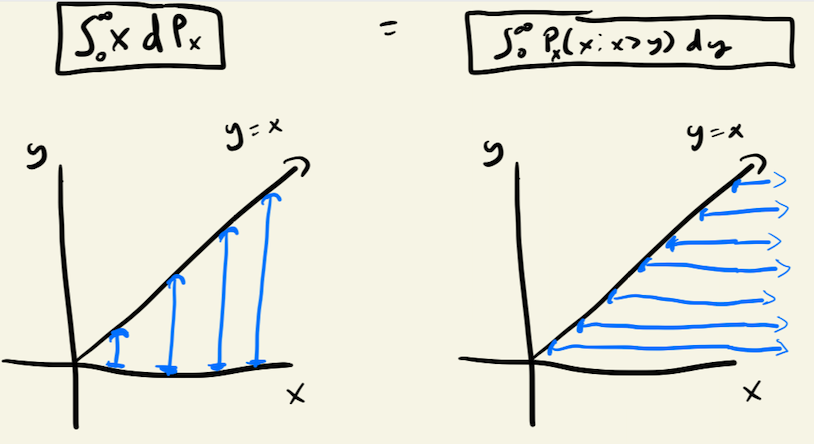
\includegraphics[width=0.9\textwidth]{images/expected_value_equals_integral_of_survival_function}
\caption{\textit{The expected value of a non-negative random variable equals the integral of its survival function.}  Note from the left that the expected value can be seen as the area under $y=x$ if the x-axis is measured with $P_X$.}
\end{figure}
\end{frame}

\end{document}



